\documentclass[]{report}
\usepackage[]{amsmath}
\usepackage[]{mathtools}
\usepackage[]{mathmod}
\usepackage[]{tikz}
\usepackage[]{listings}
\usepackage[]{amssymb}
\usepackage[]{pgfplots}
\usepackage[left=3cm,right=3cm]{geometry}

\renewcommand{\familydefault}{\sfdefault}
\renewcommand{\arraystretch}{1.5}

\title{%
    Spacetime coercive wave equation tests\\
    \large Notes for the wave equation coercive formulation 
    numerical tests}

\author{Paolo Bignardi}

\begin{document}
    \maketitle
    \chapter*{Problem description}
    \section*{Introduction}
    We want to solve the problem:
    \begin{equation}
        \begin{cases}
            u_{tt} - c^2 \Lap u = f \qquad &\text{in } Q = \Omega \times (0,T)\\
            \Grad u \cdot \normal - (\theta c)^{-1}u_t = g \qquad &\text{in } \Sigma = \partial \Omega \times (0,T) \\
            u = u_0  \qquad  & \text{in } \Omega \times \{0\} \\
            u_t = u_1 \qquad & \text{in } \Omega \times \{0\}
        \end{cases}
    \end{equation}
    To solve this problem we use the coercive formulation. See report for the actual terms of the bilinear form.

    Here we show discretization and implementation details.
    \section*{Problem geometry}
    Since we are considering the $(1+1)$-d problem, we can introduce the grid with $x$ on the horizontal axis, and $t$ on the vertical one. We discretize the space-time cylinder using rectangles.
    \begin{center}
        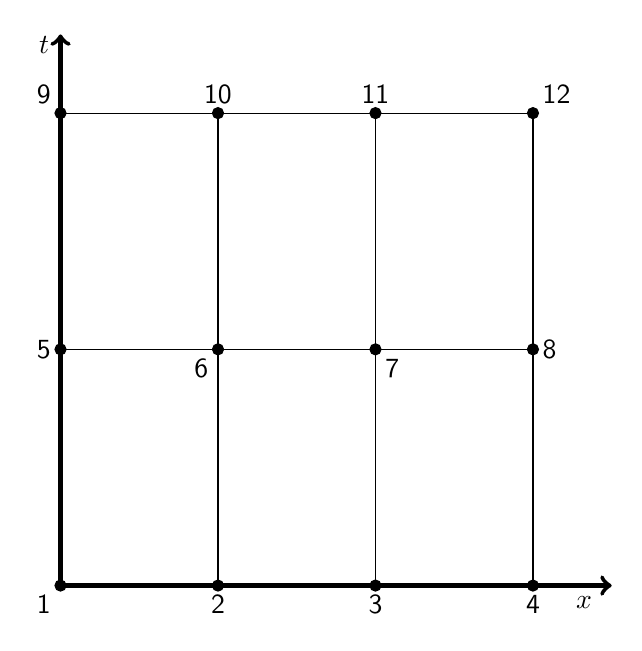
\begin{tikzpicture}% coordinates%\begin{}[]%\addplot coordinates {};%\end{}%\end{}
            \coordinate (1) at (0,0);
            \coordinate (2) at (2,0);
            \coordinate (3) at (4,0);
            \coordinate (4) at (6,0);
            \coordinate (5) at (0,3);
            \coordinate (6) at (2,3);
            \coordinate (7) at (4,3);
            \coordinate (8) at (6,3);
            \coordinate (9) at (0,6);
            \coordinate (10) at (2,6);
            \coordinate (11) at (4,6);
            \coordinate (12) at (6,6);

            \coordinate (x) at (7,0);
            \coordinate (t) at (0,7);

            \draw (1) rectangle (6);
            \draw (2) rectangle (7);
            \draw (3) rectangle (8);
            \draw (5) rectangle (10);
            \draw (6) rectangle (11);
            \draw (7) rectangle (12);

            \draw[->,ultra thick] (1)--(x) node[below, pos=.95]{$x$};
            \draw[->,ultra thick] (1)--(t) node[left, pos=.98]{$t$};
            
            \filldraw (1) circle (2pt) node[below left]{1};
            \filldraw (2) circle (2pt) node[below]{2};
            \filldraw (3) circle (2pt) node[below]{3};
            \filldraw (4) circle (2pt) node[below]{4};
            \filldraw (5) circle (2pt) node[left]{5};
            \filldraw (6) circle (2pt) node[below left]{6};
            \filldraw (7) circle (2pt) node[below right]{7};
            \filldraw (8) circle (2pt) node[right]{8};
            \filldraw (9) circle (2pt) node[above left]{9};
            \filldraw (10) circle (2pt) node[above]{10};
            \filldraw (11) circle (2pt) node[above]{11};
            \filldraw (12) circle (2pt) node[above right]{12};
        \end{tikzpicture}
    \end{center}
    Here we have numbered all the nodes of the mesh, in a \textit{left-to-right} and \textit{bottom-to-top} fashion, therefore we can compute easily the boundary nodes. In general assume we have $N_x$ space nodes, and $N_t$ time nodes.
    \begin{enumerate}
        \item Bottom boundary: $[1,\dots,N_x]$,
        \item Top boundary: $[(N_t - 1)N_x + 1, \dots, N_x N_t]$,
        \item Left boundary: $[1, N_x + 1, 2N_x + 1, \dots, (N_t - 1) N_x + 1]$,
        \item Right boundary: $[N_x, 2N_x, \dots, N_t N_x]$.
    \end{enumerate}
    All the elements of the space-time cylinder are enumerated in terms of their nodes left-right and bottom-top. In our example, the first element is stored in the first entry of an array (for now) as the tuple $(1,2,5,6)$. This needs to be consistent with the way the elements of the basis are ordered.
    \section*{1d Hermite basis}
    The basis of the element in 1d is given by
    \begin{align*}
        \hat H_1(x) &= 2x^3-3x^2+1, \\
        \hat H_2(x) &= -2x^3+3x^2, \\
        \hat H_3(x) &= x^3-2x^2+x, \\
        \hat H_4(x) &= x^3 - x^2.
    \end{align*}
    Below we explain how they are associated to the degree of freedom
    \begin{center}
        \begin{tabular}[]{|c|c|}
            \hline
            Basis function & Associated DOF \\
            \hline \hline
            $\hat{H}_1(x) = 2x^3-3x^2+1$ & $v \mapsto v(0)$ \\
            \hline
            $\hat{H}_2(x) = -2x^3+3x^2$ & $v \mapsto v(1)$ \\
            \hline
            $\hat{H}_3(x) = x^3-2x^2+x$ & $v \mapsto v'(0)$ \\ 
            \hline
            $\hat{H}_4(x) = x^3 - x^2$ & $v \mapsto v'(1)$ \\
            \hline
        \end{tabular}
    \end{center}
    \begin{center}
        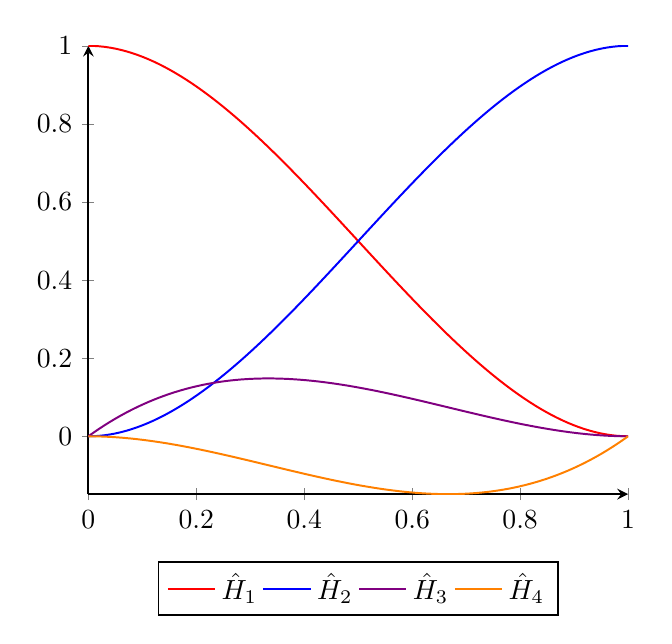
\begin{tikzpicture}
            \begin{axis}[
                axis lines = left,
                line width = .25mm,
                legend style = {at = {(.5,-.15)}, anchor=north, legend columns=-1},
                ]
            \addplot[ 
                domain = 0:1,
                samples = 100,
                color = red,
                ]
                {2*x^3-3*x^2+1};
            \addlegendentry{\(\hat{H}_1\)};
            \addplot[
                domain = 0:1,
                samples = 100,
                color = blue,
            ]   {-2*x^3+3*x^2};
            \addlegendentry{\(\hat{H}_2\)};
            \addplot[
                domain = 0:1,
                samples = 100,
                color = violet,
            ]   {x^3-2*x^2+x};
            \addlegendentry{\(\hat{H}_3\)};
            \addplot[
                domain = 0:1,
                samples = 100,
                color = orange,
            ]   {x^3-x^2};
            \addlegendentry{\(\hat{H}_4\)};
            \end{axis}
        \end{tikzpicture}
    \end{center}
    Consider the transformation $\phi$ to the reference element $[0,1]$ from a local element $[x_k, x_{k+1}]$, given by
    \begin{equation*}
        \phi(x) = \frac{x-x_k}{h}, \qquad x \in [x_k,x_{k+1}],
    \end{equation*}
    then the local basis $H_i$ is written in terms of reference basis as
    \begin{equation*}
        H_i(x) = \hat{H}_i(\phi(x)).
    \end{equation*}
    When we compute the derivatives of the local element, we need to take into account also the derivative of the transformation $\phi$
    \begin{align*}
        H'_i(x) &= \hat{H}'_i(\phi(x)) \phi'(x) = \frac{1}{h} \hat{H}'_i(\hat{x}), \\
        H''_i(x) &= \hat{H}''_i(\phi(x)) \phi'(x)^2 = \frac{1}{h^2} \hat{H}''_i(\hat{x}), \\
        H^{(k)}_i(x) &= \hat{H}^{(k)}_i(\phi(x)) \phi'(x)^k = \frac{1}{h^k}\hat{H}^{(k)}_i(\hat{x}),
    \end{align*}
    for $k \in \N$. We also need to take into account the jacobian of the trasformation when integrating over the local element. Let $\psi$ the inverse of $\phi$ defined by $\psi(\hat{x}) = h \hat{x} + x_k$. 
    \begin{align*}
        \int_{x_k}^{x_{k+1}} H_i(x)H_j(x)dx = \int_0^1 \hat{H}_i(\hat{x}) \hat{H}_j(\hat{x}) |\psi'(\hat{x})| d\hat{x} = h \int_0^1 \hat{H}_i(\hat{x}) \hat{H}_j(\hat{x}) d\hat{x}.
    \end{align*}
    {\color{red} So when construting the local matrix we need to multiply by $h$, and divide by $h$ as many times as the order of the derivative.}

    \section*{2d Hermite basis}
    To obtain the 2d Hermite basis, the simple and sensible thing to do is to construct the local operators by tensor product with the 1d operators, as seen in the next section. 
    The standard basis function is of the form:
    \begin{equation}
        H_n(x,y) = H_{j_n}(x) H_{k_n}(y), \qquad x, y \in [0,1].
    \end{equation}

    \begin{center}
        \begin{tikzpicture}[scale=4]
            \coordinate (1) at (0,0);
            \coordinate (2) at (1,0);
            \coordinate (4) at (1,1);
            \coordinate (3) at (0,1);

            \draw[] (0,0) rectangle (1,1);
            \node[below left]  (v1) at (1) {$V_1$};
            \node[below right] (v2) at (2) {$V_2$};
            \node[above left] (v3) at (3) {$V_3$};
            \node[above right]  (v4) at (4) {$V_4$};
            
            \filldraw (1) circle (.5pt);
            \filldraw (2) circle (.5pt);
            \filldraw (3) circle (.5pt);
            \filldraw (4) circle (.5pt);

            \draw (1) circle (1pt);
            \draw (2) circle (1pt);
            \draw (3) circle (1pt);
            \draw (4) circle (1pt);

            \draw[color=red] (1) circle (1.5pt);
            \draw[color=red] (2) circle (1.5pt);
            \draw[color=red] (3) circle (1.5pt);
            \draw[color=red] (4) circle (1.5pt);
        \end{tikzpicture}
        \boxed{
            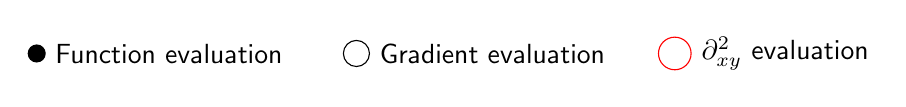
\begin{tikzpicture}[scale=4]% coordinates%\begin{}[]%\addplot coordinates {};%\end{}%\end{}
                \node[circle, draw, anchor=west, label=right:{Gradient evaluation}] at (0,-.25) { };
                \node[fill=black, circle, draw, scale = .65, anchor=west, label=right:{Function evaluation}] at (-1,-.25) { };
                \node[red, circle, draw, scale = 1.25, anchor=west, label=right:{$\partial^2_{xy}$ evaluation}] at (1,-.25) { };
            \end{tikzpicture}
        }
    \end{center}
    

    There are 4 degrees of freedom for each node, and for the vertex $V_i$ they are:
    \begin{align*}
        v &\mapsto v(V_i), \\
        v &\mapsto \partial_x v(V_i), \\
        v &\mapsto \partial_y v(V_i), \\
        v &\mapsto \partial^2_{xy} v(V_i).
    \end{align*}
    We would like to have shape funcion evaluations dofs in the first elements of the basis, and derivative as last elements globally. 
    {\itshape This is not good for the sparsity pattern of the matrix, but it should not be a problem for the solver.}
    If we take Kronecker product of the local operator matrices, we get the following order:
    \begin{align*}
        \left[
            v_1, v_2, (v_1)_x, (v_2)_x,
            v_3, v_4, (v_3)_x, (v_4)_x,
            (v_1)_y, (v_2)_y, (v_1)_{xy}, (v_2)_{xy},
            (v_3)_y, (v_4)_y, (v_3)_{xy}, (v_4)_{xy}
            \right].
    \end{align*}
    We need to define a function that maps node numbers to their respective degrees of freedom. Given that we have $N_x + 1$ nodes in the $x$ direction, and $N_t + 1$ nodes in the $t$ direction, then we have $N_n = (N_x + 1) (N_t + 1)$ number of nodes in the mesh. The mapper function is defined as
    \begin{align*}
        M: i \mapsto (i, i + N_n, i + 2 N_n, i + 3 N_n).
    \end{align*}
    When assembling the global stiffness matrix, we need to take into account that matrix computed with Kronecker product are not ordered in the way we want. {\color{red} So we either reorder the Kronecker matrix, or we reorder the mapper function after computing the degrees of freedom for the element.}
    
    \section*{Reference operators}
    To construct the operators of the bilinear form, introduce the local operators for the space and time component, $S$ is for space, $T$ is for time. 

    
    Apices will be used to denote the order of derivation for the trial and test functions: for example, $S^{00}$ is the \textbf{local mass matrix} for the space component. In general $S^{ij}$ is the local matrix associated to the local operator
    \begin{equation*}
        \int_{\hat{R}} \partial_i u \cdot \partial_j v dx,
    \end{equation*}
    letting $u$ and $v$ vary among all the space local basis functions, where $\hat{R}$ is the reference space element.
    Similarly $T^{ij}$ is associated to the local operator 
    \begin{equation*}
        \int_0^1 \partial_i u \cdot \partial_j v dt,
    \end{equation*}
    letting $u$ and $v$ vary among all the time local basis functions.
    
    {\bfseries Important note: in Kronecker product the first element is associated to the column terms, wherease the second is associated to the rows.} So when computing Kronecker product first comes the time component matrix (vertical component - i.e. columns) and then the space component matrix (horizontal component - i.e. columns).
    
    \subsection*{$H^1(Q)$ terms}
    Scalar products of the $H^1(Q)$ space are easy to compute.
    \begin{align*}
        &\int_Q u_tv_t = T^{11} \otimes S^{00}\\
        &\int_Q \Grad u \cdot \Grad v =  T^{00} \otimes S^{11}
    \end{align*}

    \subsection*{Least square term}
    Least square term comes from the integral $\int_Q Wu Wv$. Expanding, we get
    \begin{equation*}
        \int_Q \left[ u_{tt} v_{tt} - c^2 u_{tt} \Lap v - c^2 v_{tt} \Lap v +c^4 \Lap u \Lap v \right],
    \end{equation*}
    Each terms is collected in the table below
    \begin{center}
        \begin{tabular}[]{|c||c|c|}
            \hline
                        & $u_{tt}$    & $\Lap u$ \\
            \hline \hline
            $v_{tt}$    & $S^{00} \otimes T^{22}$ & $S^{20} \otimes T^{02}$ \\
            \hline
            $\Lap v$    & $S^{02} \otimes T^{20}$ & $S^{22} \otimes T^{00}$ \\
            \hline
        \end{tabular}
    \end{center}

    \subsection*{$\int_Q {Z}u {W}v$ term}
    Expanding all terms we get
    \begin{equation*}
        \int_Q Zu Wv = ...
    \end{equation*}
    Note the there are variable terms that need to be taken into account, so we consider the local integral for the local matrix.
    \begin{center}
        \begin{tabular}[]{|c||c|c|c|}
            \hline
                        & $u_{t}$ & $t u_t$ & $\vec{x} \cdot \Grad u$ \\
            \hline \hline
            $v_{tt}$    & $h^{-3} T^{22} \otimes S^{00} $ & $h^{-3}  T^{02} \otimes S^{20}$ \\
            \hline
            $\Lap v$    & $h^{-3} T^{20} \otimes S^{02}$ & $h^{-3}  T^{00} \otimes S^{22}$ \\
            \hline
        \end{tabular}
    \end{center}

    \begin{align*}
        &\int_Q t u_t v_{tt} =  T^{12}_t \otimes S^{00} \\
        &\int_Q t u_t \Lap v = T^{10}_t \otimes S^{02}  \\
        &\int_Q u_t v_{tt} = T^{12} \otimes S^{00}  \\
        &\int_Q u_t \Lap v =  T^{10} \otimes S^{02}  \\
        &\int_Q \vec{x} \cdot \Grad u v_{tt} = T^{02} \otimes S^{10}_x \\
        &\int_Q \vec{x} \cdot \Grad u \Lap v = T^{00}  \otimes S^{12}_x 
    \end{align*}

    \subsection*{Variable operators}
    Operators of the form 
    \begin{equation*}
        \int_Q \vec{x} \cdot \Grad u v_{tt}, \qquad \int_Q t u_t v_{tt}, ...
    \end{equation*}
    must be computed carefully. Taking $u$ and $v$ to be trial and test function respectively, we can still split the integral, and obtain the following expression
    \begin{equation*}
        \int_{\Omega} \vec{x} H_{i_k}'(x) H_{i_l}(x) dx \cdot \int_0^T H''_{j_k}(t) H_{j_l}(t) dt.
    \end{equation*}
    Hence we only have to compute the matrix associated to the 1d problem of the first integral, and then Kronecker-multiply by the respective other. The first integral depends on the element we compute it on, indeed
    \begin{align*}
        \int_{x_i}^{x_{i+1}} x H'_{i_k}(x) H_{i_l}(x) dx &= \int_0^1 h (\hat{x}h + x_i) H'_{i_k}(\hat{x}h + x_i) H_{i_l}(\hat{x}h + x_i) d\hat{x} \\
        &= h \int_0^1 \hat{x} H'_{i_k}(\hat{x})H_{i_l}(\hat{x}) d\hat{x} + x_i \int_0^1 H'_{i_k}(\hat{x})H_{i_l}(\hat{x}) d\hat{x}.
    \end{align*}
    To compute those contributions in the global matrix, we need to sum those terms over their respective degrees of freedom. For the case considered above the code would look like this
    \begin{verbatim}
        for e in elms
            p = first(e)                                # get the pivot index
            x_p, y_p = nodes[p]                         # get its coordinates
            stencil = ...                               # compute the DOFs stencil
            KlocVar = kron(h*S_10x + x_p*S_10, T_20)    # compute local matrix
            K[stencil, stencil] += KlocVar              # update global matrix
        end
    \end{verbatim}

    We need to take into account the $h_x$ and $h_t$ factors. Note that for both reference matrix $S^{ij}$ and $T^{kl}$ we multiply by $h_x$ and $h_t$ respectively. Then the derivation reduce the order of $h_x$ and $h_t$; multiplier $\vec{x} \cdot$ and $t$ increase by one the exponent.

    So local operators are:
    \begin{center}
        \begin{tabular}[]{|c|c|}
            \hline
            Reference operator on $[0,1]$ & Local operator on $[x_n,x_{n+1}] \times [t_m, t_{m+1}]$\\
            \hline \hline
            $T^{kl} \otimes S^{ij}$ & $h_x^{1 - i - j} T^{kl} \otimes h_t^{1 - k - l}S^{ij}$ \\
            \hline
            $T^{kl} \otimes S_x^{ij}$ & $h_t^{1 - k - l} T^{kl}\otimes \left[h_x^{2 - i - j} S_x^{ij} + x_{n} h_x^{1 - i - j} S^{ij}\right]$ \\
            \hline
            $T_t^{kl} \otimes S^{ij}$ & $ \left[h_t^{2 - k - l} T_t^{kl} + t_{m} h_t^{1 - k - l} T^{kl}\right] \otimes h_x^{1 - i - j} S^{ij}$ \\
            \hline
        \end{tabular}
    \end{center}

    \section*{Boundary operators}
    Over the boundary we have several boundary terms, and we can use the same assemble strategy to compute those boundary terms. 
    We can cycle over the boundary $\Sigma$ and the boundary $\Omega_0$ and $\Omega_T$, and sum over and over the local stiffness matrix of the boundary terms, which can be constructed. These will be a 4\times4 matrix that can be constructed appropriately.

    \subsection*{\Sigma\ boundary term}
    Since the space domain is only one-dimensional, the gradient term are actually only derivatives. Also the boundary is only given by two points, so effectively we only have to integrate over $\{x_0\}\times [0,T]$ and over $\{x_1\} \times [0,T]$. Effectively, this amounts to evaluating the space terms of the integral, and multiplying by the time derivative operators. For example, consider the term
    \begin{equation*}
        \int_{\Sigma} Zv u_t = \int_{\Sigma} \vec{x} \cdot \Grad v u_t + \beta(t-T^*) v_t u_t
    \end{equation*}
    We can split the integral into space and time part, and consider the basis functions $H_i(x,t) = H_{j_i}(x)H_{k_i}(t)$, (and consider for simplicity only the boundary $x_0$)
    \begin{equation*}
        \int_0^T H'_{k_n}(t)H'_{k_m}(t) \cdot \int_{\{x_0\}} H_{j_n}(x) H_{j_m}(x) = \left(\int_0^T H'_{k_n}(t)H'_{k_m}(t)\right) \cdot H_{j_n}(x_0)H_{j_m}(x_0)
    \end{equation*}
    Note that the product $ H_{j_n}(x_0) H_{j_m}(x_0)$ is always 0 except when $j_n = j_m$. To make things simpler, we can use the Kronecker product and use the same strategy as for any other element.
    Hence the local operator of the example becomes:
    \begin{equation*}
        S^{00}\Big|_{x_0} \otimes T^{11}
    \end{equation*}

    Note that $S^{00}\Big|_{x_0}$ has only a 1 element on the diagonal in position (1,1). Whereas, the matrix $S^{00}\Big|_{x_1}$ as a 1 element in position $(2,2)$. The fact that evaluation matrices only have a single non-zero element, the Kronecker matrix has 16 non-zeros, which are associated to the right degrees of freedom.

    \section*{Degrees of freedom mapping}
    In this section we describe the mapping from the global degrees of freedom to the reference element ones. We want to produce a vector of indices that maps columns and rows of the local stiffness matrix to the global matrix.

    Recall the mapping function for each node $i$. Consider the element given by the nodes $I = (i_1, i_2, i_3, i_4)$, then we can compute the degrees of freedom of the element as
    \begin{align*}
        I \otimes \bm{1}_4 + N_n \bm{1}_4 \otimes (0,1,2,3),
    \end{align*}
    where $\bm{1}_n$ is the n-vector containing all ones. The above vector is just
    \begin{align*}
        \big(M(i_1), M(i_2), M(i_3), M(i_4)\big).
    \end{align*}
    Though, the local matrix we build with Kronecker products do not reflect this ordering of the elements, so we need to reorder the vector. The order we take the element of the vector above is given by
    \begin{verbatim}
        [1, 5, 2, 6, 9, 13, 10, 14, 3, 7, 4, 8, 11, 15, 12, 16],
    \end{verbatim}
    and this yields a vector that select the degrees of freedom in the prescribed order
    \begin{align*}
        \left[
            v_1, v_2, (v_1)_x, (v_2)_x,
            v_3, v_4, (v_3)_x, (v_4)_x,
            (v_1)_y, (v_2)_y, (v_1)_{xy}, (v_2)_{xy},
            (v_3)_y, (v_4)_y, (v_3)_{xy}, (v_4)_{xy}
            \right].
    \end{align*}
    As an example, consider the element defined by nodes $(1,2,4,5)$ and assume we have $N_n = 9$, then unordered vector is
    \begin{verbatim}
        [1, 10, 19, 28, 2, 11, 20, 29, 4, 13, 22, 31, 5, 14, 23, 32]
    \end{verbatim}
    and the mapping vector is
    \begin{verbatim}
        [1, 2, 10, 11, 4, 5, 13, 14, 19, 20, 28, 29, 22, 23, 31, 32].
    \end{verbatim}

    \section*{Load vector}
    To compute the load vector, we use Gauss quadrature. We just need to compute quadrature points \texttt{xq} and weights \texttt{wq} for the reference element. Then we evaluate the Hermite basis function, its first and second derivative and combine them using Kronecker products to assemble the term $\operator{Z} v$ and $\operator{W} v$.
    
    When computing the derivative of the basis function, we need to take into account the constant $h_x$ and $h_t$ coming up because of the derivation. 

    Then for each operator we have a matrix that contains 16 columns (one for each basis function) and \texttt{nq * nq} rows, depending on the number of quadrature points on the reference square. This matrix must be multiplied column-wise with the vector of evaluation of the function $f$ over the element.

    To integrate then we multiply column-wise with the weights \texttt{wqxt} which are the Kronecker product of the local weights in each direction (multiplied by $h_x$ and $h_t$ for their respective direction). 
    Then sum across the columns, and use the mapper function described in the previous section to map the local load vector to the global load vector.
    \section*{Solution evaluation}


    \chapter*{Matlab functions rundown}

    \section*{Appendix A: FEM matrix assembly}
    Consider $\Omega = [0,1]^2$ as the domain, and the following subdivision:
    \begin{center}
        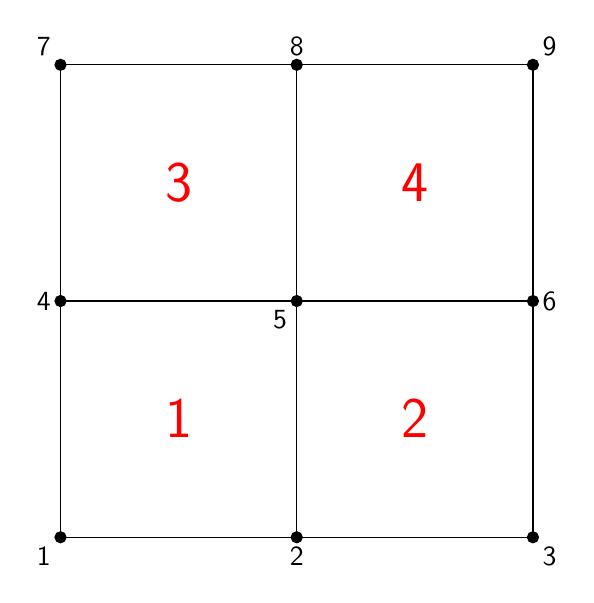
\begin{tikzpicture}
            \coordinate (1) at (0,0);
            \coordinate (2) at (3,0);
            \coordinate (3) at (6,0);
            \coordinate (4) at (0,3);
            \coordinate (5) at (3,3);
            \coordinate (6) at (6,3);
            \coordinate (7) at (0,6);
            \coordinate (8) at (3,6);
            \coordinate (9) at (6,6);

            \draw (0,0) rectangle (3,3) node[pos=.5, color=red, font=\huge]{1};
            \draw (3,3) rectangle (6,6) node[pos=.5, color=red, font=\huge]{4};
            \draw (3,0) rectangle (6,3) node[pos=.5, color=red, font=\huge]{2};
            \draw (0,3) rectangle (3,6) node[pos=.5, color=red, font=\huge]{3};

            \path (1) node[below left] {1};
            \path (2) node[below] {2};
            \path (3) node[below right] {3};
            
            \path (4) node[left] {4};
            \path (5) node[below left] {5};
            \path (6) node[right] {6};
            
            \path (7) node[above left] {7};
            \path (8) node[above] {8};
            \path (9) node[above right] {9};
            
            \filldraw (1) circle (2pt);
            \filldraw (2) circle (2pt);
            \filldraw (3) circle (2pt);
            \filldraw (4) circle (2pt);
            \filldraw (5) circle (2pt);
            \filldraw (6) circle (2pt);
            \filldraw (7) circle (2pt);
            \filldraw (8) circle (2pt);
            \filldraw (9) circle (2pt);
        \end{tikzpicture}    
    \end{center}
    Assume we have a local matrix called $A$, which is easy to compute. Now construct the \textit{connectivity matrix} which has in each column the list of vertices of the element.
    \begin{equation*}
        T = \begin{pmatrix*}
            1 & 2 & 4 & 5 \\
            2 & 3 & 5 & 6 \\
            4 & 5 & 7 & 8 \\
            5 & 6 & 8 & 9
        \end{pmatrix*}
    \end{equation*}
    Now, assembly the global matrix by 
    \begin{verbatim}
        for e = 1:n_elems
            el_nodes = T[:,e]
            K[el_nodes,el_nodes] = K[el_nodes,el_nodes] + A
        end
    \end{verbatim}
    
    How do we treat more general elements? \dots

    Suppose we have a finite element that has $k$ local degree of freedom, then the situation is similar as if we had multiple nodes in the same point in space. So for each node of the mesh, we have $k$ columns (and rows) corresponding to the degrees of freedom over that node. The stencil to access the global matrix is not just a column of the connectivity matrix, but it is a more general vector, that depends on how the basis functions are ordered!!

    \section*{Appendix B: Load vector assembly}

\end{document}